\documentclass[transmag]{IEEEtran}
\usepackage{latexsym}
\usepackage{graphicx}
\usepackage{amsfonts,amssymb,amsmath}
\usepackage{hyperref}
\usepackage{subfig}
\usepackage{amsmath}
\usepackage{titlesec}
\usepackage{bbold}
\usepackage{listings}
\usepackage{pdfpages}
\usepackage{lastpage}
\usepackage{lipsum}
\usepackage{hyperref}
\usepackage{array}
\usepackage{tabularx}
\usepackage{multirow}
\usepackage{float}
\usepackage{siunitx}
\graphicspath{ {../notebook/img/} }
\def\BibTeX{{\rm B\kern-.05em{\sc i\kern-.025em b}\kern-.08em T\kern-.1667em\lower.7ex\hbox{E}\kern-.125emX}}
%\markboth{$>$ REPLACE THIS LINE WITH YOUR PAPER IDENTIFICATION NUMBER $<$}
%{$>$ REPLACE THIS LINE WITH YOUR PAPER IDENTIFICATION NUMBER $<$}
\begin{document}



\title{Predicting Ethereum Price Change Using News Articles}

\author{\IEEEauthorblockN{Ashutosh Bansal}
\textit{19323385}
\and
\IEEEauthorblockN{Ming Jun Lim}
\textit{21337483}
\and
\IEEEauthorblockN{Markus Scully}
\IEEEauthorblockA{
\textit{16321114}}}




\maketitle
\thispagestyle{plain}
\pagestyle{plain}


%\section{INTRODUCTION}
\section{Introduction}
% explain the problem and why it is interesting
\IEEEPARstart{T}{he} cryptocurrency market have witnessed an explosion in the recent years with Bitcoin\footnote{\ Bitcoin is the first well known cryptocurrency started in the late 2000s} hitting lots of new time high and many investors moving to this trading space \cite{huy2019predicting}. With the internet constantly evolving, social networking sites such as Facebook, Twitter, Instagram and etc have become a means of communication between people. There have been researches in text sentiment analysis to predict price changes for Bitcoin \cite{huy2019predicting}\cite{sattarov2020forecasting} as Bitcoin is considered a dominant cryptocurrency. However many other cryptocurrency have been developed and have been in demand such as Ethereum \footnote{\ Ethereum is a programmable blockchain and cryptocurrency described as Ether}. The project will be tackling Ethereum market price by estimating if the future price increases or decreases based on text processing sourced from the web such as social networking sites and forums. The problem is converted into a classfication problem by comparing the future market price with current market price instead of a regression problem of estimating the future market price. Can news or posts of Ethereum articles really affect the market price?

\noindent The input to our algorithm is text sourced web scrapers on social networking sites. We then compare several machine learning methods such as k-Nearest Neighbours (kNN), logistic regression and Support Vector Machine (SVM) to output a predicted label, +1 if price increased or -1 if price decreased.

\section{Dataset and Features}
\noindent The dataset consists of Ethereum related articles and class labels gathered from Twitter, Reddit and Binance\footnote{\ Binance is one of the largest cryptocurrency exchange} over the last four years. Data from Twitter and Reddit are merged with a similar column names: \emph{date} \emph{content} and \emph{popularity}.

\subsection{Data Source}
\label{data_source}
% twitter
\subsubsection{Twitter}
\noindent Twitter provides an official API for accessing tweets but access to this requires an approval process \cite{twitter_api_docs}. Instead, the open-source Python library snscrape \cite{snscrape_git} was used to collect 240 tweets for each day in the range January 2017 to October 2021, filtered by search for the word "Ethereum". The popularity content for each tweet was calculated by summing together the number of retweets, likes and replies it received. This popularity value was then normalised by dividing it by the highest popularity value of all collected tweets.

% reddit
\subsubsection{Reddit}
\noindent Reddit is divided into smaller sub-communities relating to specific themes called "subreddits". The subreddits "EtherMining", "Cryptocurrency", "Cryptocurrencies", "CryptoMarkets", "EthTrader", "Ethereum", and "Bitcoin" were selected as source of data because of their relevancy. Comments posted on submission on each of these subreddits were scraped using the library psaw which itself pulls data from service Pushshift. The popularity value of each comment was determined by its "karma" value, a measure of how much positive feedback it has received from other users of the site. Up to 240 comments were scraped per subreddit per day, for a maximum of 1680 per day if that many comments had actually been posted.

% Binance
\subsubsection{Binance}
\noindent Binance provides a set of API \cite{binance_web_socket}, WebSocket endpoints available to collect live data and old historical data \cite{binance_public_data}. Monthly trade data of ETHUSDT\footnote{\ ETHUSDT is a symbol for Ethereum and USDT pair, 1 USDT is 1 USD.} symbol is collected from August, 2017 to October, 2021 with a total of 657,446,190 data points. These data points are processed by calculating the average price by days and discretizing the continuous values into +1 and -1 class labels by comparing it with the previous day resulting into 1,537 data points.

\begin{figure}[h!]
    \centering
    \subfloat[Mean price against Data points]{{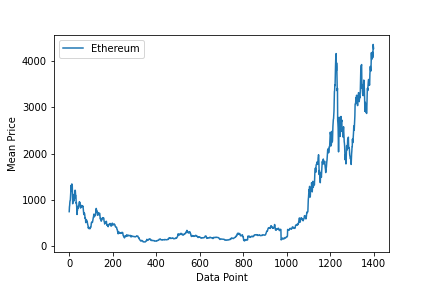
\includegraphics[width=0.5\columnwidth]{binance_mean_price.png} }}%
%    \qquad
    \subfloat[Count against labels]{{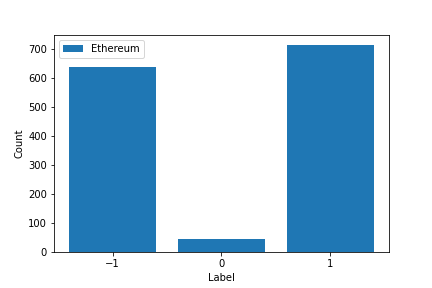
\includegraphics[width=0.5\columnwidth]{binance_label.png} }}%
    \caption{Overview of Binance dataset collected}%
    \label{fig:binance_overview}%
\end{figure}

\noindent There is another class label "0" in figure \ref{fig:binance_overview}.b. This is due to the first day of every month unable to calculate different with the day before. It was set to "-1" to have binary labels.

\subsection{Feature Extraction}

\noindent Several pre-processing steps are applied. The first step is tokenization, splitting input character sequences into tokens. The endings of the tokens are chopped of by stemming. The tokens are pruned using a set of stop words as they contribute little to no information such as words "is", "the", "a", etc. Tokens appearing frequently and rarely were also pruned through the \verb|min_df| and \verb|max_df| parameters in tokenization, this step was very important to reduce the feature size. The algorithm uses Natural Language Toolkit \verb|nltk| library providing stemming functions such as \verb|PorterStemmer| and a list of stopwords \verb|nltk.corpus.stopwords.words("english")|. Some general pre-processing on text data from \cite{sattarov2020forecasting} were applied onto our dataset consisting of:
\begin{itemize}
  \item Converting all words to lower case.
  \item Removing words containing numbers.
  \item Removing symbols from words ("\#","\@@").
  \item Removing words containing non\-english characters.
\end{itemize}

\noindent These sequence of tokens are mapped to a feature vector using the bag of words model, the model consists of hyper-parameter n-grams and cross validation for 1-gram single token and 2-gram pairs of token are evaluated in section ???. The n-gram hyper-parameter enables model to preserve some word ordering but feature vector size can grow quickly.

\section{Methods}
\label{methods}

\subsection{k-Nearest Neighbours}
\noindent K-Nearest Neighbours (kNN) is an instance-based model that uses training data to make predictions. Given a feature vector $x$ to make prediction, the distance of $x$ is calculated with all training data, selects k closest training points and assigns majority label of the neighbours for classification problem. kNN requires a distance function, hyper-parameter \emph{k} of neighbours to be considered, weighting of neighbour points and method for aggregating \emph{k} neighbour points $N_k$. 


% distance metric
\begin{equation}
\label{eqn:knn_euclidean}
d(x^{(i)},x) = \sqrt[2]{ \sum^n_{j=1} (x^{(i)}_j - x_j)^2 }
\end{equation}
% weighting of neighbours
\begin{equation}
\label{eqn:knn_uniform}
w^{(i)} = 1
\end{equation}
\begin{equation}
\label{eqn:knn_gaussian}
w^{(i)} = e^{-\gamma d(x^{(i)},x)^2}
\end{equation}
\begin{equation}
\label{eqn:knn_classification}
sign(\frac{ \sum_{i \in N_k} w^{(i)} y^{(i)} }{ \sum_{ i \in N_k} w^{(i)} })
\end{equation}

\noindent Equation (\ref{eqn:knn_euclidean}) is Euclidean distance commonly used for kNN.
Equation (\ref{eqn:knn_uniform}) uniform and equation (\ref{eqn:knn_gaussian}) Gaussian are methods weighting of neighbour points. For the Gaussian weighting, training points further away from the target variable \emph{i} are attached with lesser weight compared to nearer ones. Equation (\ref{eqn:knn_classification}) is the method for aggregating \emph{k} neighbour points $N_k$, it is a majority vote when uniform weighting neighbour points is used.

\subsection{Logistic Regression}
\noindent Logistic regression is a linear model that uses $sign(\theta^Tx)$ to quantize continuous values to output labels $+1$ when $\theta^Tx > 0$ and $-1$ when $\theta^Tx < 0$. Decision boundary is $\theta^Tx = 0$ and dataset is considered to be linearly separable when classes can be separated by decision boundary. 

% weighted sum
\begin{equation}
\label{eqn:logistic_weighted_sum}
\theta^Tx = \theta_0x_0 + \theta_1x_1 + ... + \theta_nx_n
\end{equation}
% logistic cost function
\begin{equation}
\label{eqn:logistic_cost}
J(\theta) = \frac{1}{m} \sum^m_{i=1} log (1 + e^{-y^{(i)}\theta^Tx^{(i)}})
\end{equation}
\noindent Equation (\ref{eqn:logistic_weighted_sum}) is the weighted combination of the input features and weight. Equation (\ref{eqn:logistic_cost}) is the cost function for logistic regression. The learning algorithm uses gradient descent to minimises cost function $J(\theta)$ by pushing weights $\theta$ towards direction away from decision boundary to minimise loss. The cost function $J(\theta)$ is convex and gradient descent iterates by moving downhill reaching the minimum point.


% L1
\begin{equation}
\label{eqn:logistic_l1}
R(\theta) = \sum^n_{j=1} |\theta_j|
\end{equation}
% L2
\begin{equation}
\label{eqn:logistic_l2}
R(\theta) = \theta^T\theta = \sum^n_{j=1}\theta^2_j
\end{equation}
\noindent Regularisation can be added to logistic regression by using penalty term in the cost function such as L1 penalty equation (\ref{eqn:logistic_l1}) and L2 penalty equation (\ref{eqn:logistic_l2}). These penalty terms uses hyper-parameter by affecting minimisation of first term or penalty term in learning. L1 penalty encourages sparsity of solution, causing weights to be 0. L2 penalty encourages weights $\theta$ to have smaller values.


\subsection{Support Vector Machine}

\noindent Support Vector Machine (SVM) is a classifier similar to logistic regression, the prediction uses $sign(\theta^Tx)$ and the output is mapped to $+1$ and $-1$. 

\begin{equation}
\label{eqn:hinge_loss_function}
max(0,1-y\theta^Tx))
\end{equation}

\noindent The main difference lies in the cost function as shown in equation (\ref{eqn:hinge_loss_function}), SVM uses a "hinge" loss function. The cost function of SVM is non-smooth. There is no penalty to all values of $\theta$ when the prediction is correct. Penalty for regularisation is mandatory for SVM to get sensible behaviour due to $\theta^Tx$, scaling the term up will output loss of 0. Example prediction is $+1$ and label is $+1$, Equation \ref{eqn:hinge_loss_function} will be $max(0, 1 - (+1)(+45)) = 0$
\begin{equation}
\label{eqn:svm_penalty}
\theta^T\theta = \sum^n_{j=1} \theta^2_j
\end{equation}
\begin{equation}
\label{eqn:svm_cost_function}
J(\theta) = \frac{1}{m}\sum^m_{i=1}max(0,1-y^{(i)}\theta^Tx^{(i)})+\frac{\theta^T\theta}{C}
\end{equation}
Equation \ref{eqn:svm_penalty} is the sum of squares elements in parameter vector that penalises large values of $\theta$. Equation \ref{eqn:svm_cost_function} is the final SVM cost function. The first term depends on how much the model predicts training data and $C$ in the penalty term is a hyper-parameter affecting training in minimising which terms in the equation. The learning selects $\theta$ that minimises cost function $J(\theta)$.


\section{Experiments}
\noindent 5-fold cross validation were used to select hyper-parameters for models mentioned in section \ref{methods}. The dataset metioned in section \ref{data_source} were grouped by dates resulting with a total of 1400 data points from \emph{2018-01-01} to \emph{2021-10-31}. The dataset was split into training and test set with a ratio of $80:20$. The baseline models used to evaluate against these models were a model always predicting the most common class and a model randomly predicting class.

\label{sec:metric}
\noindent The choice of metric used for evaluation $F_1$ score, recall, precision and accuracy. The ROC curve and AUC were also plotted and compared with other classifiers and baseline.

% f1 score
\begin{equation}
\label{eqn:f1_score}
F_1 \textnormal{score}\ = \frac{2TP}{2TP+FN+FP}
\end{equation}
% recall
\begin{equation}
\label{eqn:recall}
\textnormal{recall}\ = \frac{TP}{TP+FN}
\end{equation}
% precision
\begin{equation}
\label{eqn:precision}
\textnormal{precision}\ = \frac{TP}{TP+FP}
\end{equation}

\noindent Equation (\ref{eqn:f1_score}) is the $F_1$ score metric measuring the harmonic mean of precision and recall. Equation (\ref{eqn:recall}) is the recall metric. Equation (\ref{eqn:precision}) is the precision metric. \emph{TP} represent true positive, \emph{FP} represents false positive, \emph{TN} represents true negative and \emph{FN} represents false negative.

\subsection{k-Nearest Neighbours}
\noindent The k-Nearest Neighbours (KNN) has a hyper-parameter \emph{k}. Cross validation was used to determine \emph{k} from a range $[0..700]$ with interval of 10. The distance metric used for kNN was Euclidean distance described in equation (\ref{eqn:knn_euclidean}). The weighting of neighbour points used is uniform and method for aggregating \emph{k} neigbour points $N_k$ are described in equation (\ref{eqn:knn_uniform}) and equation (\ref{eqn:knn_classification}).

\begin{figure}[h]
	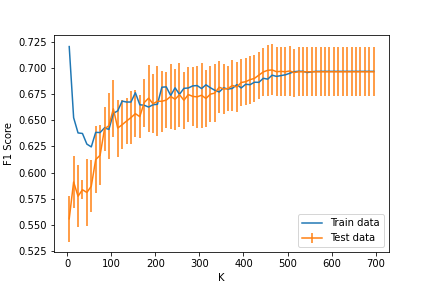
\includegraphics[width=\columnwidth]{knn_cv_k.png} 
    \caption{Error plot kNN with range of \emph{k} parameters}%
    \label{fig:knn_k}%
\end{figure}
\noindent Figure (\ref{fig:knn_k}) is an error plot of cross validation in the range of \emph{k}. The selected \emph{k} hyper-parameter is 465 as shown in the figure. Smaller values of \emph{K} such as 1 are over-fitting as the $F_1$ score  for train data is higher than test data.

\subsection{Logistic Regression}
\noindent The L2 penalty term described in equation (\ref{eqn:logistic_l2}) is used for the logistic regression. The range of C values used are from \num{1e-10} to \num{9.51e-08} with incremental of \num{5e-09} to select hyper-parameter for the penalty term through cross validation.

\begin{figure}[h]
	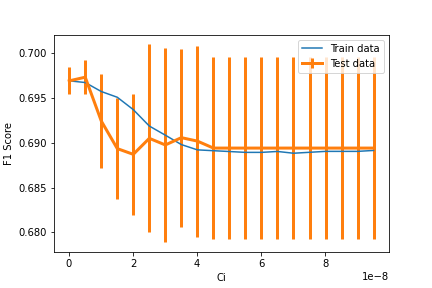
\includegraphics[width=\columnwidth]{logistic_cv_ci.png} 
    \caption{Error plot logstic regression with range of C values}%
    \label{fig:logistic_c}%
\end{figure}

\noindent Figure (\ref{fig:logistic_c}) is an error plot of cross validation in the range of C. The selected C value hyper-parameter is \num{3.51e-08} as shown the figure. Such small figures were used to increase weighting of the penalty term to prevent over-fitting.


\subsection{Support Vector Machine}
\noindent The range of C values used are similar to logistic regression from \num{1e-10} to \num{9.51e-08} with incremental of \num{5e-09} to select hyper-parameter for the penalty term in equation (\ref{eqn:svm_cost_function}) through cross validation.

\begin{figure}[h]
	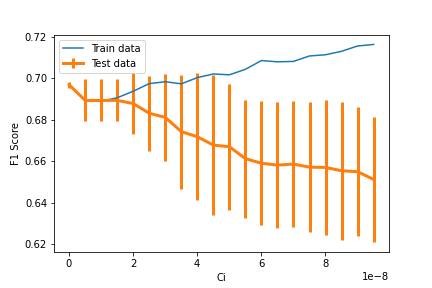
\includegraphics[width=\columnwidth]{svm_cv_ci.png} 
    \caption{Error plot SVM with range of C values}%
    \label{fig:svm_c}%
\end{figure}

\noindent Figure (\ref{fig:svm_c}) is an error plot of cross validation in the range of C. The selected C value hyper-parameter is \num{1.01e-8} as shown in the figure. The weight of the penalty is controlled by hyper-parameter C, higher value results in lower weight likewise for lower value as described by equation (\ref{eqn:svm_cost_function}). Values after \num{1.01e-8} is over fitting as the $F_1$ score for test data keeps decreasing while train data increases.

\section{Results}

\noindent The evaluation metrics mentioned in section (\ref{sec:metric}) are described in table (\ref{tab:results}). Logistic regression and SVM models have the highest $F_1$ score for class $+1$ with the same value of $0.74$, slightly higher than the most common baseline model with a value of $0.73$. The random baseline model has the highest $F_1$ score for class $-1$ with a value of $0.53$ while other models were below $0.18$. KNN, logistic regression and SVM models have very high recall score for $+1$ above $0.96$ but very low recall score for $-1$ class below $0.10$. The precision of $+1$ class is similar throughout the models with random baseline model having highest score of $0.64$. Logistic regression and SVM models have the highest precision score for $-1$ class with the same value $0.80$, while KNN performed the worse than random baseline model. Logistic regression and SVM models have the highest accuracy score with the same value of $0.61$ while KNN has a lower score compared to the most common baseline model. SVM has the highest AUC score of $0.592$ and KNN the lowest AUC of $0.495$.

\begin{figure}[h]
	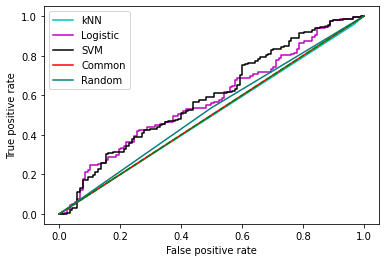
\includegraphics[width=\columnwidth]{roc_curve.png} 
    \caption{ROC curve plot of all algorithms}%
    \label{fig:results_roc}%
\end{figure}

%\begin{table*}[!bh]
\begin{table*}[!h]

\begin{tabularx}{\textwidth}{|| p{5cm} | X | X | X | X | X | X | X | X ||}
\hline
\multirow{2}{*}{\textbf{Algorithm}}  & \multicolumn{2}{c|}{\textbf{F1 Score}} & \multicolumn{2}{c|}{\textbf{Recall}} & \multicolumn{2}{c|}{\textbf{Precision}} & \multirow{2}{*}{\textbf{Accuracy}} & \multirow{2}{*}{\textbf{AUC}} \\ 
\cline{2-7}
& \centering +1& \centering -1 & \centering +1 & \centering -1 & \centering +1 & \centering -1 & & \\ 
\hline
Most Common (baseline) & 0.73 & 0.00 & 1.00 & 0.00 & 0.58 & 0.00 & 0.58 & 0.500 \\
\hline
Random (baseline) & 0.57 & 0.53 & 0.51 & 0.61 & 0.64 & 0.47 & 0.55 & 0.519 \\
\hline
k-Nearest Neightbours (kNN) & 0.72 & 0.06 & 0.96 & 0.03 & 0.58 & 0.36 & 0.57 & 0.495 \\
\hline
Logistic Regression & 0.74 & 0.18& 0.98 & 0.10 & 0.60 & 0.80 & 0.61 & 0.578 \\
\hline
Support Vector Machine (SVM) & 0.74 & 0.18 & 0.98 & 0.10 & 0.60 & 0.80 & 0.61 & 0.592 \\
\hline

\hline
\end{tabularx}
\caption{Results of algorithms with evaluation metrics}
    \label{tab:results}%
\end{table*}


\section{Discussion}
\noindent The logistic regression and SVM model relies heavily on the penalty term due to small \emph{C} hyper-parameter, both these models use the same L2 penalty term in equation (\ref{eqn:logistic_l2}). As the weight of penalty term increases, the learning algorithm minimises this term resulting in very similar scores between logistic regression and SVM models. Table (\ref{tab:top10words}) describes the top 10 words and weights of logistic regression and SVM models. The list has the same words but differs slightly in ranking and weights are similar. Based on human intuition, these list of words are not informative in determining a price increase or decrease.

\begin{figure}[h]
\begin{center}
\begin{tabular}{|l|ll|ll|}
\hline
\multicolumn{1}{|c|}{\multirow{2}{*}{\textbf{Rank}}} & \multicolumn{2}{c|}{\textbf{Logistic Regression}} & \multicolumn{2}{c|}{\textbf{SVM}}    \\ \cline{2-5} 
\multicolumn{1}{|c|}{}                               & \multicolumn{1}{l|}{Word}        & Weight         & \multicolumn{1}{l|}{Word} & Weight   \\ \hline
1                                                    & \multicolumn{1}{l|}{it}          & 8.32e-05       & \multicolumn{1}{l|}{it}   & 7.49e-05 \\ \hline
2                                                    & \multicolumn{1}{l|}{you}         & 7.66e-05       & \multicolumn{1}{l|}{you}  & 6.77e-05 \\ \hline
3                                                    & \multicolumn{1}{l|}{on}          & 6.05e-05       & \multicolumn{1}{l|}{on}   & 6.23e-05 \\ \hline
4                                                    & \multicolumn{1}{l|}{eth}         & 5.18e-05       & \multicolumn{1}{l|}{eth}  & 5.34e-05 \\ \hline
5                                                    & \multicolumn{1}{l|}{your}        & 4.39e-05       & \multicolumn{1}{l|}{your} & 4.22e-05 \\ \hline
6                                                    & \multicolumn{1}{l|}{my}          & 4.09e-05       & \multicolumn{1}{l|}{my}   & 3.82e-05 \\ \hline
7                                                    & \multicolumn{1}{l|}{but}         & 3.69e-05       & \multicolumn{1}{l|}{fee}  & 3.80e-05 \\ \hline
8                                                    & \multicolumn{1}{l|}{do}          & 3.66e-05       & \multicolumn{1}{l|}{do}   & 3.74e-05 \\ \hline
9                                                    & \multicolumn{1}{l|}{fee}         & 3.65e-05       & \multicolumn{1}{l|}{but}  & 3.57e-05 \\ \hline
10                                                   & \multicolumn{1}{l|}{have}        & 3.57e-05       & \multicolumn{1}{l|}{have} & 3.50e-05 \\ \hline
\end{tabular}
\end{center}
\caption{List of Top 10 words and weights of logistic regression and SVM models}
    \label{tab:top10words}
\end{figure}

\noindent The ROC curve shows balance between true and false positives rate and each model's ROC curve is plotted in figure (\ref{fig:results_roc}). Logistic regression and SVM models performed slightly better than the baseline models, KNN performed worse than the baseline models. Logistic regression performed better than SVM model at lower false positive rate. SVM model performed better than logistic regression at higher false positive rate.

\begin{figure}[h]
\begin{center}
\begin{tabular}{|l|l|}
\hline
\multicolumn{1}{|c|}{\textbf{Word}} & \multicolumn{1}{c|}{\textbf{Frequency}} \\ \hline
the                                 & 1983224                                 \\ \hline
to                                  & 1483911                                 \\ \hline
and                                 & 1054822                                 \\ \hline
it                                  & 999065                                  \\ \hline
is                                  & 904312                                  \\ \hline
you                                 & 892661                                  \\ \hline
of                                  & 881741                                  \\ \hline
that                                & 682975                                  \\ \hline
in                                  & 657324                                  \\ \hline
for                                 & 558993                                  \\ \hline
http                                & 531703                                  \\ \hline
thi                                 & 503092                                  \\ \hline
ethereum                            & 445926                                  \\ \hline
on                                  & 443100                                  \\ \hline
be                                  & 433659                                  \\ \hline
bitcoin                             & 374686                                  \\ \hline
are                                 & 367675                                  \\ \hline
have                                & 359111                                  \\ \hline
not                                 & 348293                                  \\ \hline
if                                  & 347963                                  \\ \hline
\end{tabular}
\end{center}
\caption{List of top 30 most frequent words in the dataset}
    \label{tab:top30words}
\end{figure}

\noindent Table (\ref{tab:top30words}) lists the top 30 most frequent word in the dataset after preprocessing. There is large differences between frequency of words in the dataset with least common word "lolol" having a frequency of 145.




\section{Summary}








\bibliographystyle{plain}
\bibliography{bibliography.bib}


%\newpage\null\thispagestyle{empty}\newpage

\end{document}
